\documentclass{standalone}
\usepackage{pgfplots}
\usetikzlibrary{intersections}
\usepgfplotslibrary{fillbetween}
\pgfplotsset{compat=1.7}

\begin{document}
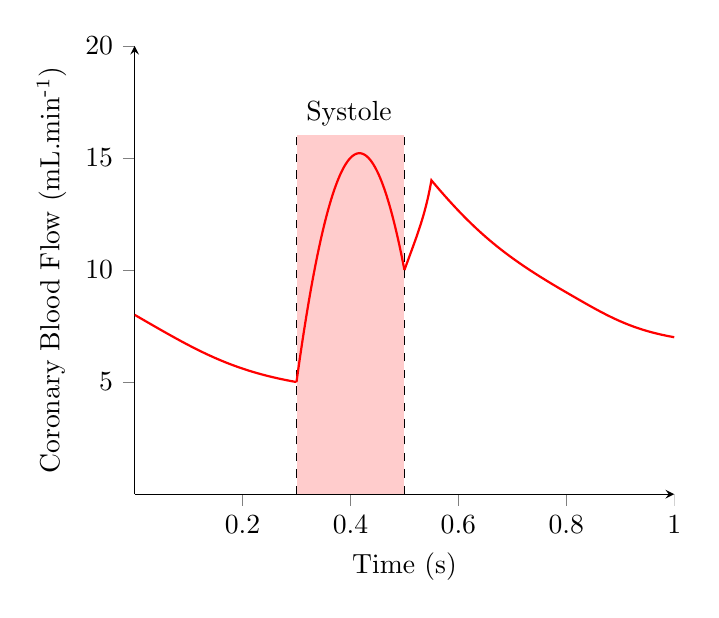
\begin{tikzpicture}


\begin{axis}[
        axis lines=middle,
        grid style={none},
	ymin = 0,
	ymax = 20,
	xmin = 0,
	xmax =1,
	 ylabel near ticks,
	xlabel near ticks,
        xlabel=Time (s),
        ylabel=Coronary Blood Flow (mL.min\textsuperscript{-1}),
        tick align=outside,
        enlargelimits=false,
legend pos= north west,
legend style={font=\small, cells={align=left}}]

\draw[name path=left, black, thin, dashed] (axis cs: 0.3,0) -- (axis cs: 0.3,16) node[pos=1, black, above right]{Systole};
\draw[name path=right, black, thin, dashed] (axis cs: 0.5,0) -- (axis cs: 0.5,16);
\addplot[fill=red,opacity=0.2] fill between [of=left and right];

%\plot[domain=0:0.3, red, thick,samples=500] {16.67*x^2 - 21.67*x + 0};
\draw[thick, red] (axis cs: 0,8) to[out=-30, in=170] (axis cs: 0.3, 5);
\plot[domain=0.3:0.5, red, thick,samples=500] { -750*x^2 + 625*x - 115};
\draw[thick, red] (axis cs: 0.5,10) to[out=70, in=-100] (axis cs: 0.55, 14) to[out=-50, in=150] (axis cs: 0.8, 9) to[out=-30, in=170] (axis cs: 1,7);

\end{axis}

\end{tikzpicture} 
\end{document}